
\subsection{Patrick Modeling}

To assess whether using a surface-specific data frame (``feature'') is the best strategy for predicting tennis matches, we created a second data frame that includes surface-specific variables as well as tournament-specific features, such as wins for each tournament on the ATP tour. To analyze the importance of the different variables in predicting our target variable ``PlayerA\_Wins'', we calculated the 20 most important variables of the new data frame using standard machine learning models:
%
\begin{itemize}
\item Decision Tree (DT),
\item Random Forest (RF),
\item Ada Boost (AB),
\item Gradient Boosting (GB), and
\item Neural Network (NN).
\end{itemize}

%
\begin{figure}[h]
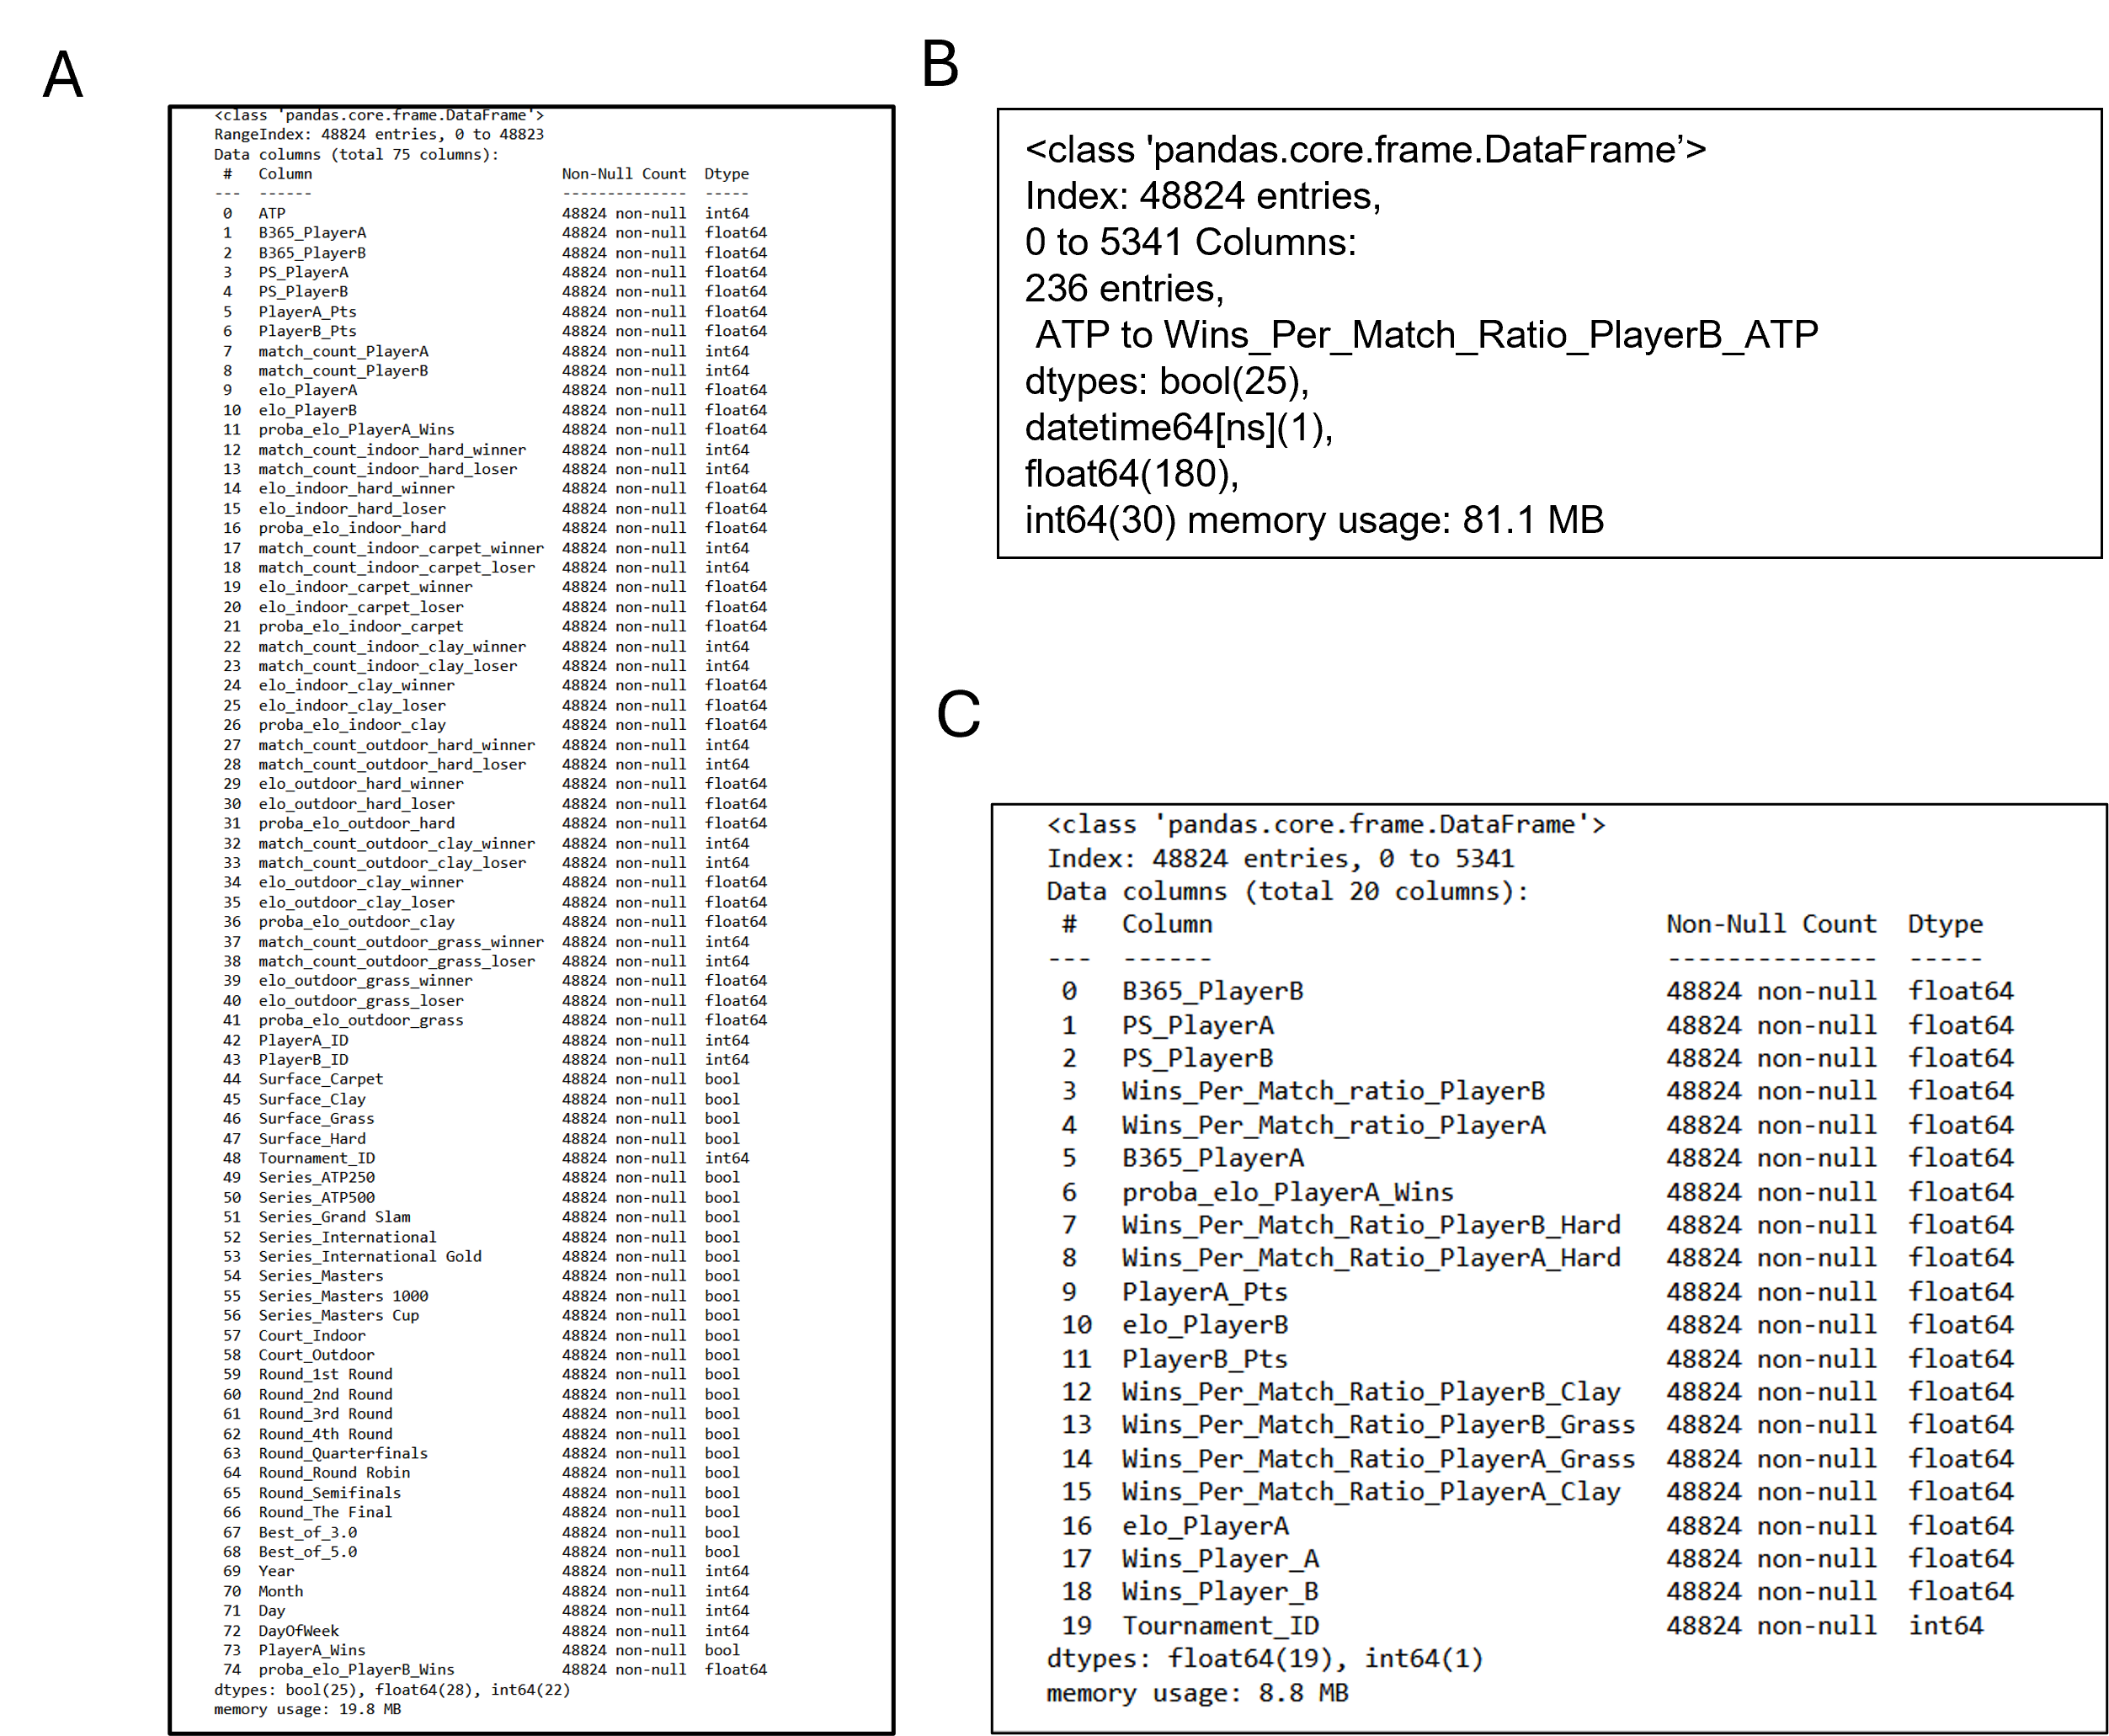
\includegraphics[width=\textwidth]{pictures/dataframes_patrick.png}
\caption{Data frames. A)  The Initial data frame. B) Engineered Data frame with 236 features, a detailed list of all the variables of this data frame can be found at additional data section of this document. C) Data frame containing top 20 features calculated from Random Forest model with the engineered data frame to predict.}
\label{dataframes_patrick}
\end{figure}
%

The images (\ref{most_important_ada}, \ref{most_important_gb}, \ref{most_important_rf}, \ref{most_important_df} )
 indicate that all machine learning algorithms used share a common set of important features for predicting the target variable 'Player A wins.' Notably, across all features presented to the algorithms, the odds from Pinnacle Sports appear to be the most influential, followed by the individual win-per-match ratio (see Table 1). Additionally, the win-match ratio on the four different surfaces emerges as particularly significant in predicting the outcome of a tennis match.

%
\begin{figure}[h]
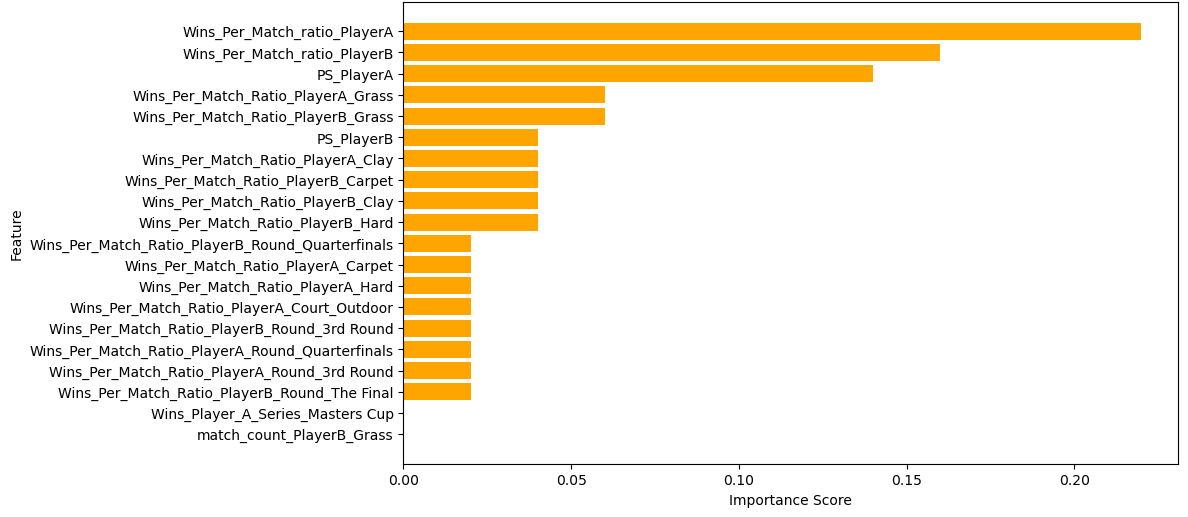
\includegraphics[width=\textwidth]{pictures/most_important_ada.png}
\caption{AdaBoost: Top 20 features predicting the target variable Player A wins.}
\label{most_important_ada}
\end{figure}
%
For AdaBoost the most important feature to predict the target variable are the wins per match ratio of each player.

%
\begin{figure}[h]
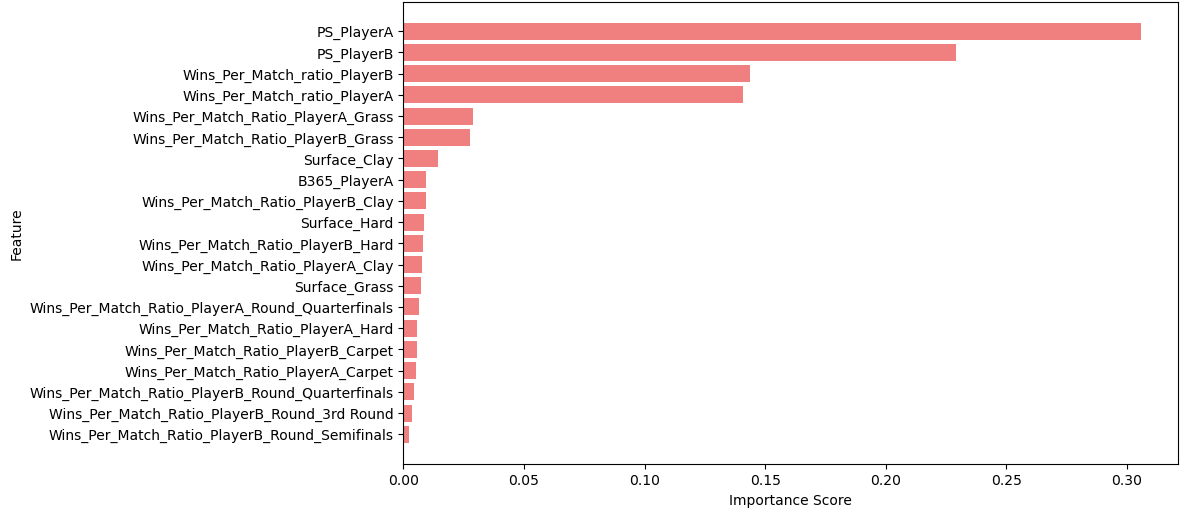
\includegraphics[width=\textwidth]{pictures/most_important_gb.png}
\caption{Gradient Boosting: Top 20 features predicting the target variable Player A wins.}
\label{most_important_gb}
\end{figure}
%
The odds of Pinnacle sports are of major importance to predict the outcome for the Gradient Boosting algorithm. 
%
\begin{figure}[h]
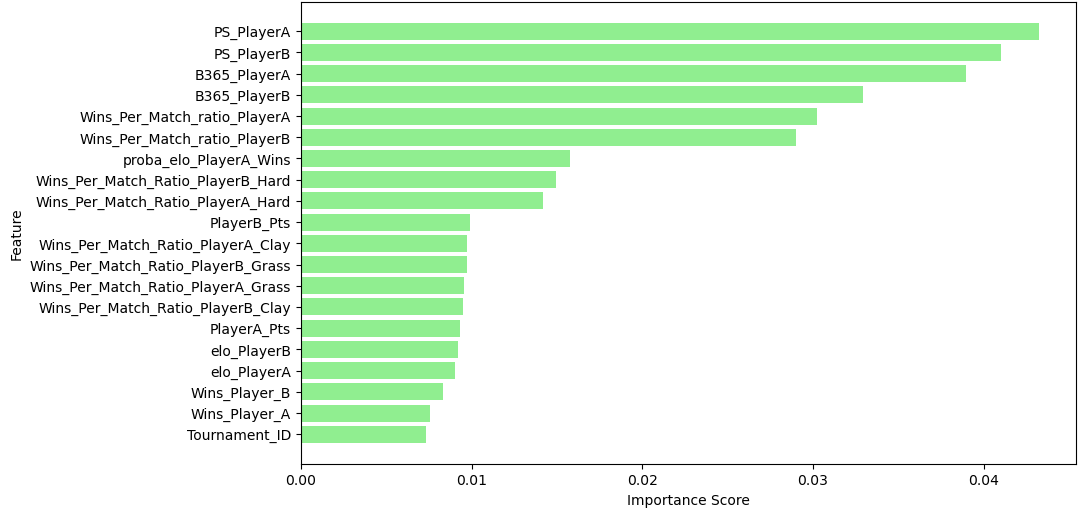
\includegraphics[width=\textwidth]{pictures/most_important_rf.png}
\caption{Random Forest: Top 20 features predicting the target variable Player A wins.}
\label{most_important_rf}
\end{figure}
%
Like the Gradient Bosting algorithm, the Random Forest algorithm highly relies on the odds of Pinnacle sports to predict the winner of the tennis match. 
%
\begin{figure}[h]
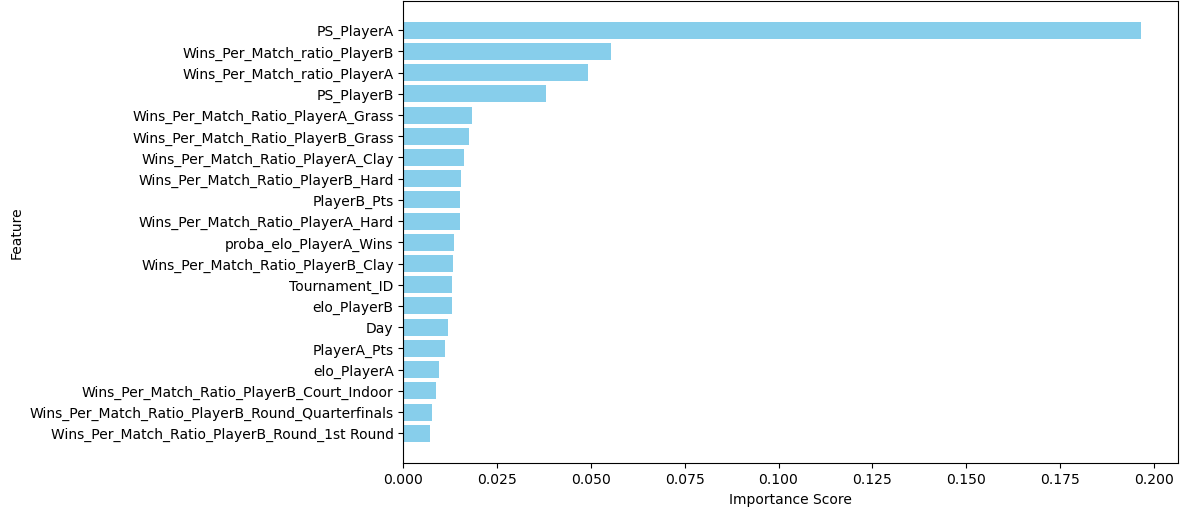
\includegraphics[width=\textwidth]{pictures/most_important_dt.png}
\caption{Decision Tree: Top 20 features predicting the target variable Player A wins.}
\label{most_important_df}
\end{figure}
%
The Decision Tree algorithm heavily relies on the odds from Pinnacle Sports, with the win-match ratios of Player A and Player B ranking second and fourth in importance, respectively.
In summary, it can be concluded that the odds from the bookmaker, along with the win-match ratios of each individual player on different surfaces, are the most critical features for predicting tennis match outcomes. Additionally, player points (word ranking system points), Elo ratings, and specific win-match ratios for particular tournaments also emerge as significant factors in predicting match outcomes.

\begin{table}[h]
\centering
\caption{Top 10 features predicting if Player A wins among DT,RF,AB, GB}
\begin{tabular}{|c|l|}
\hline
\textbf{Feature \#} & \textbf{Top 10 Features among all models} \\
\hline
1 & PS\_PlayerA \\
2 & Wins\_Per\_Match\_ratio\_PlayerB \\
3 & Wins\_Per\_Match\_ratio\_PlayerA \\
4 & PS\_PlayerB \\
5 & Wins\_Per\_Match\_Ratio\_PlayerA\_Grass \\
6 & Wins\_Per\_Match\_Ratio\_PlayerB\_Grass \\
7 & Wins\_Per\_Match\_Ratio\_PlayerA\_Clay \\
8 & Wins\_Per\_Match\_Ratio\_PlayerB\_Hard \\
9 & Wins\_Per\_Match\_Ratio\_PlayerA\_Hard \\
10 & Wins\_Per\_Match\_Ratio\_PlayerB\_Clay \\
\hline
\end{tabular}
\end{table}

The accuracy scores of all four standard ML algorithms, trained with their 20 most important features from the data frame, range between 65\% (Decision Tree) and 76\% (Gradient Boosting). In summary, it can be concluded that with Random Forest, AdaBoost, and Gradient Boosting, three out of four tennis matches can be correctly predicted (\ref{accuracy_score_models}, \ref{confusion_matrix} ).

%
\begin{figure}[h]
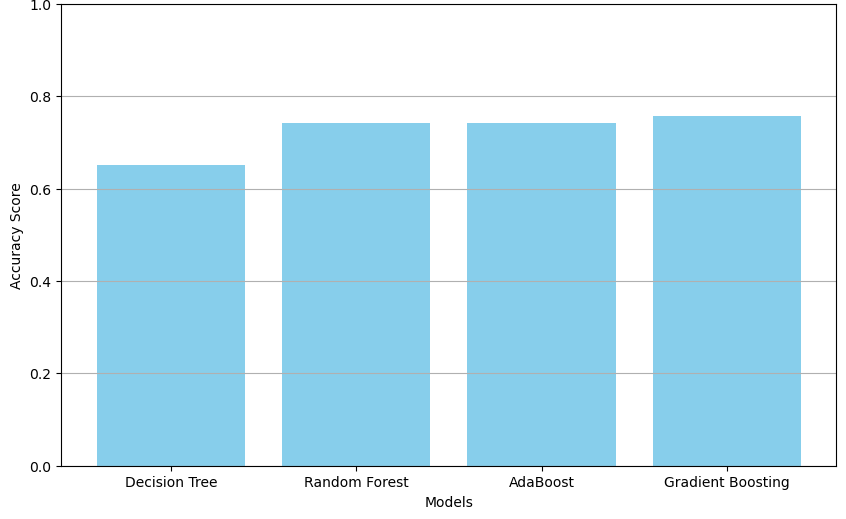
\includegraphics[width=\textwidth]{pictures/accuracy_score_models.png}
\caption{Accuracy scores of the Decision Tree, Random Forest, AdaBoost and Gradien Boosting for the Top 20 features data frame. Decision Tree: 0.65, Random Forest: 0.74, AdaBoost: 0.74 and Gradient Boosting: 0.76.}
\label{accuracy_score_models}
\end{figure}
%
To verify the calculated accuracy score for each model, we generated a confusion matrix for each( \ref{confusion_matrix} ). The data within the confusion matrices are consistent with the accuracy scores obtained. Approximately 75\% of the matches are correctly predicted (either Player A wins or loses), while about 2\% are wrongly predicted. There is no observable tendency indicating that the algorithm favors one outcome over the ot 
%
\begin{figure}[h]
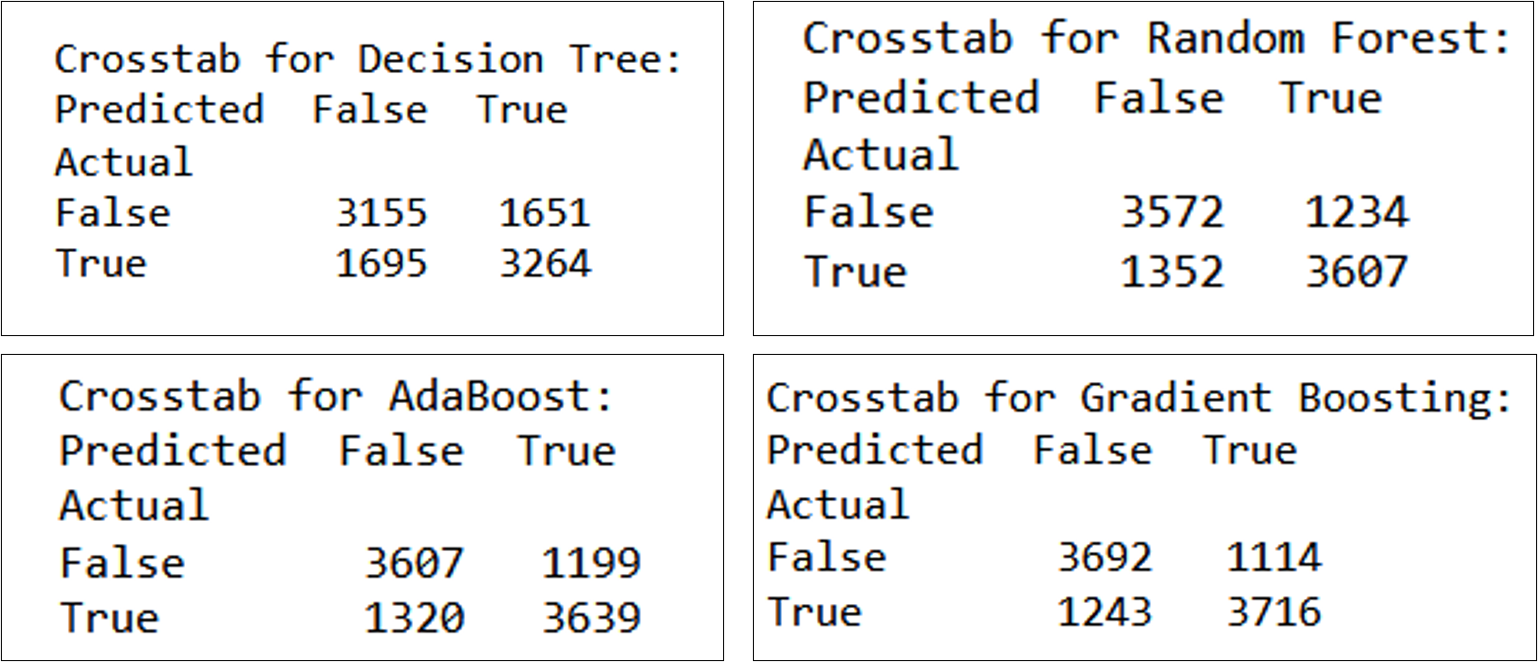
\includegraphics[width=\textwidth]{pictures/confusion_matrix.png}
\caption{Accuracy scores of the Decision Tree, Random Forest, AdaBoost and Gradien Boosting for the Top 20 features data frame. Decision Tree: 0.65, Random Forest: 0.74, AdaBoost: 0.74 and Gradient Boosting: 0.76.}
\label{confusion_matrix}
\end{figure}
%

%
\begin{figure}[h]
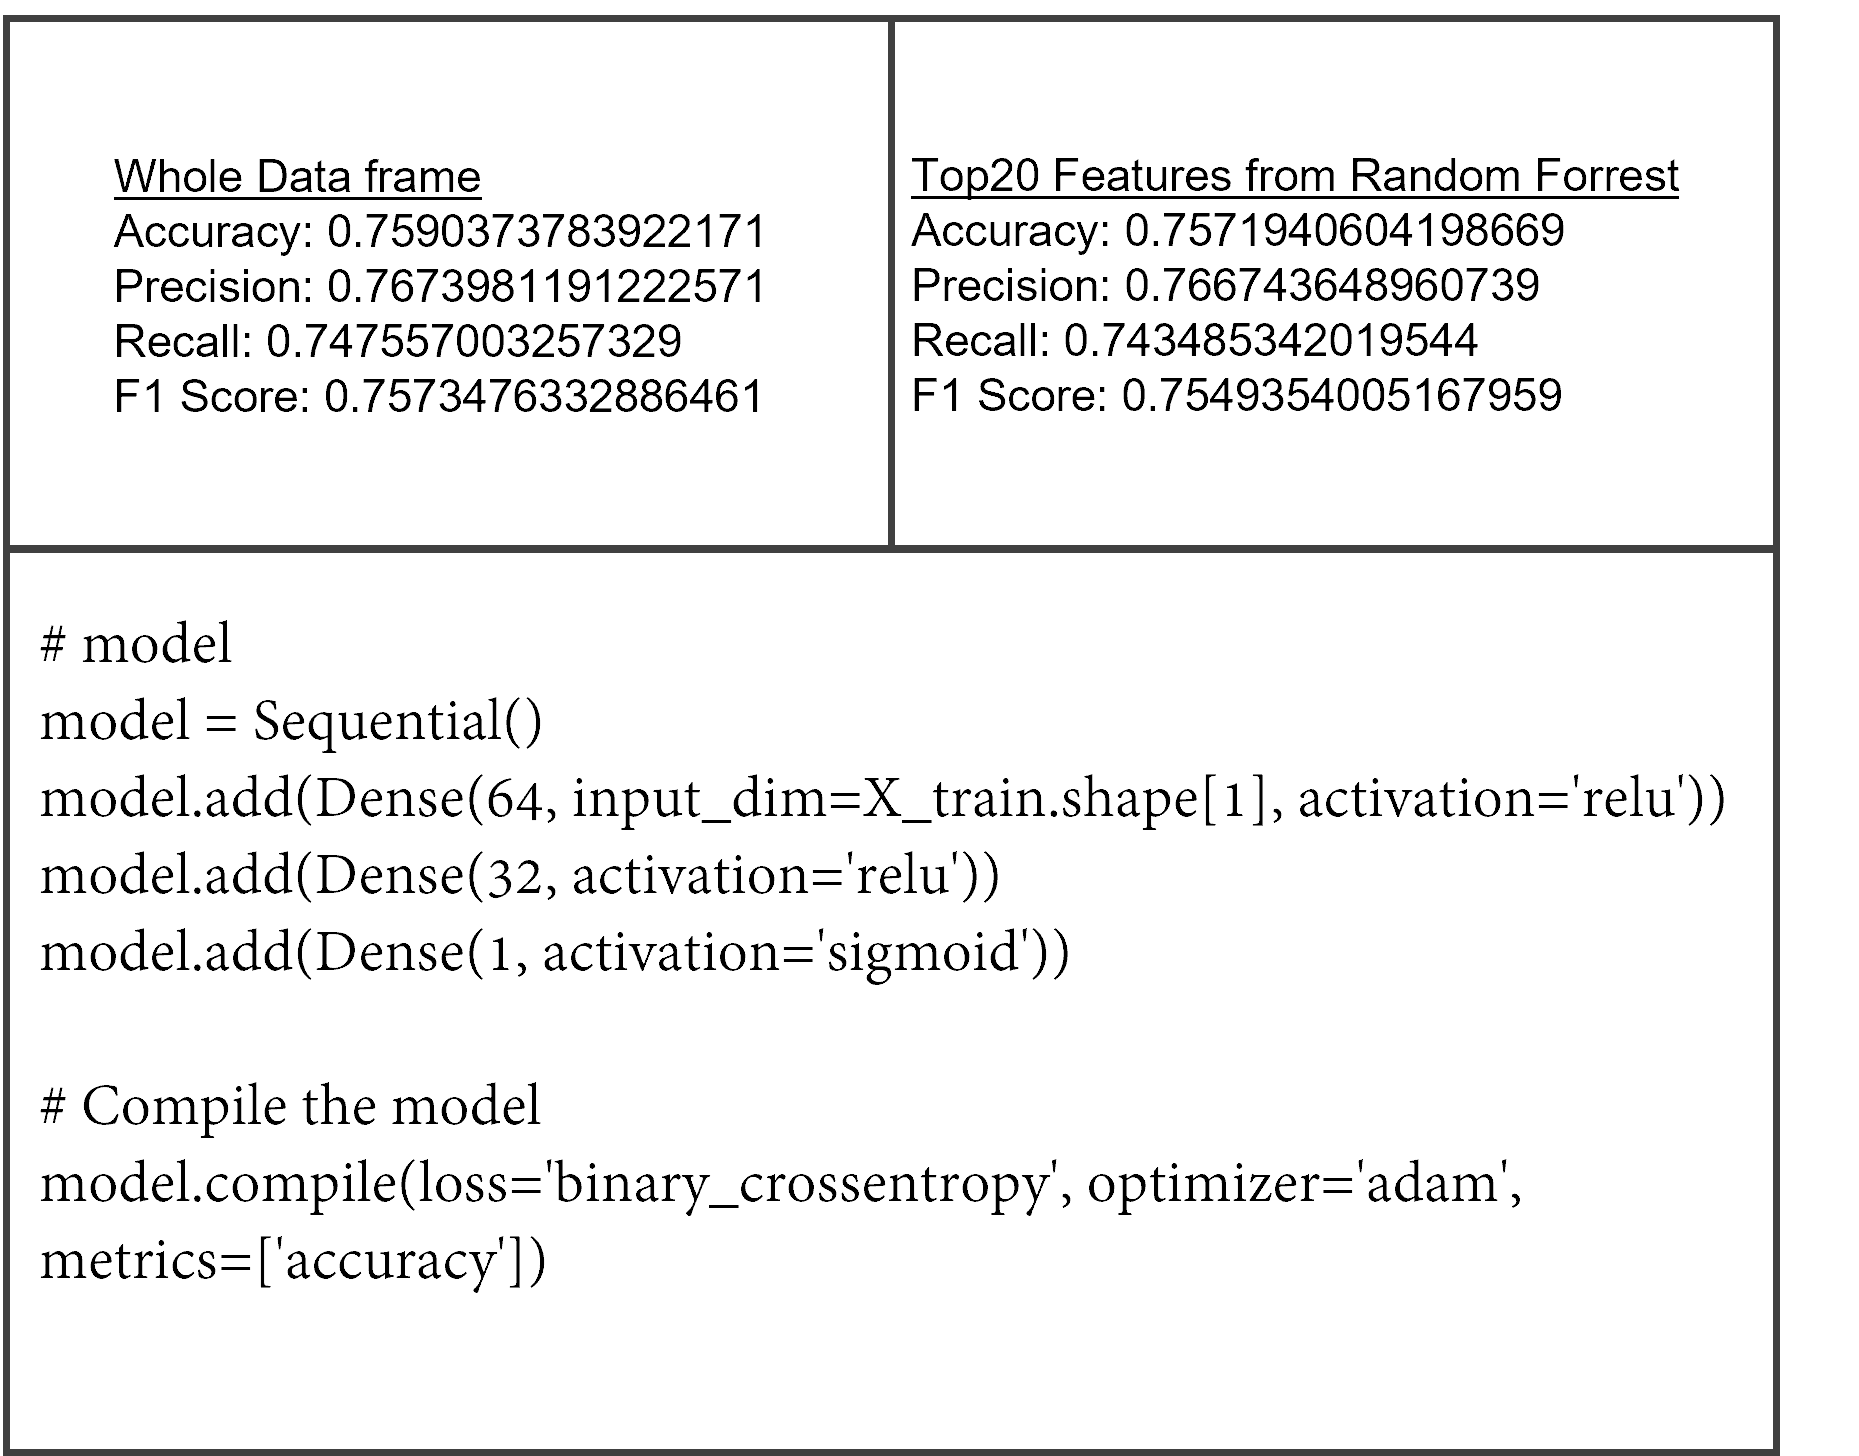
\includegraphics[width=\textwidth]{pictures/nn_model.png}
\caption{Prediction with Neural Network: A simple neural network has been trained with the Keras / Tensorflow library with the top 20 features from Random Forest to predict our target variable.}
\label{nn_moodel}
\end{figure}
%

%
\begin{figure}[h]
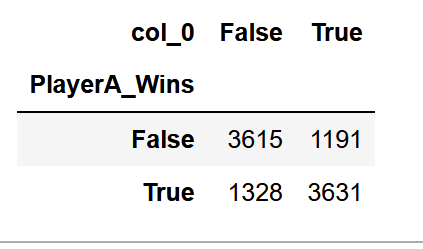
\includegraphics[width=\textwidth]{pictures/confusion_matrix_nn.png}
\caption{Confusion matrix of neural network prediction. The confusion matrix shows the predicted data plotted against the real data}
\label{confusion_matrix_nn}
\end{figure}
%

\subsection{Betting Strategy Patrick}
Our goal was not only to predict tennis matches but also to generate virtual profits with our predictions. We placed 1 unit of virtual money on each predicted game and utilized the odds from Pinnacle Sports to calculate our return on investment (ROI). After betting on 9765 tennis matches, we found that all our standard algorithms resulted in a negative ROI ( \ref{betting_strategy}). Despite our models correctly predicting 3 out of 4 tennis matches, we were unable to achieve a positive net amount of money after betting using the bookmaker's odds.
%
\begin{figure}[h]
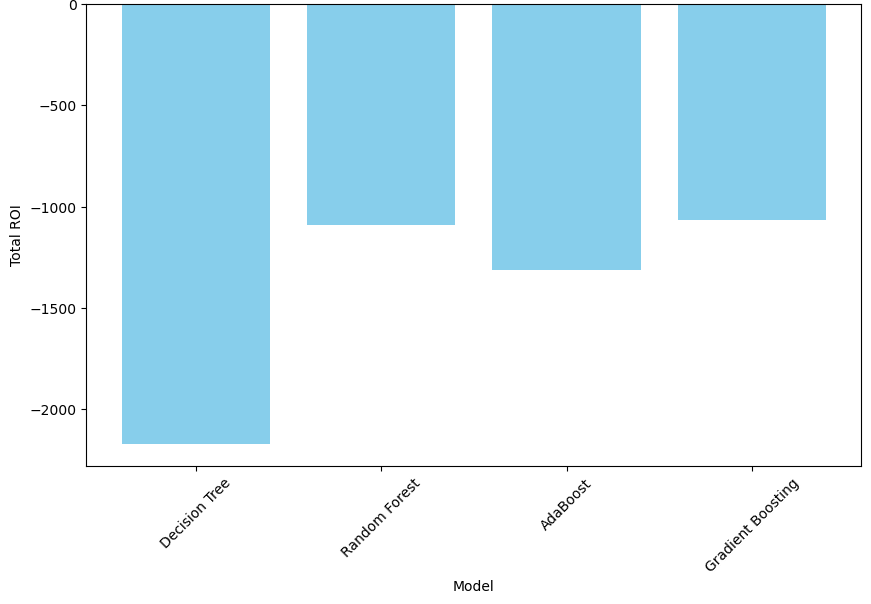
\includegraphics[width=\textwidth]{pictures/betting.png}
\caption{Return of investment after betting 1 unit on each predicted match by our algorithm.}
\label{betting_strategy}
\end{figure}
%

%
\subsection{Summary and Outlook Patrick}

\textbf{Summary and Outlook:}
We were able to train five different models that can correctly predict three out of four tennis matches. Furthermore, we identified the most important features for correctly predicting the outcome of a tennis match. Unfortunately, the prediction accuracy of about 75\% is not enough to generate a positive return on investment (ROI) using the odds from Pinnacle Sports. We also attempted to train our models on matches where both players have a high difference in Elo ratings, making it easier for the algorithm to correctly predict the winner (Data not shown). Although this strategy significantly improves the prediction accuracy, the odds on those games were so low that we wouldn’t achieve any positive ROI by betting on them. Since bookmakers' odds are designed to ensure a positive net income for the bookmaker in the long run, we should be cautious about including them in our model training. The odds set by bookmakers inherently favor the bookmaker and may negatively influence our prediction model. For future prediction models, we should not rely on bookmaker odds and instead focus more on the Elo system as well as calculated features such as a player's specific win ratio against an opponent. It might also be beneficial to aggregate important features into a single variable, such as the win ratio per match at a specific tournament and round. Another way to improve our models would be to utilize advanced neural networks like recurrent neural networks, especially Long Short-Term Memory (LSTM) networks, which incorporate time variables into their calculations and could enhance our prediction model